\chapter{Crypto.Types.Random}
This package provides randomly generated values to the calling programs.
\section{API}\label{Read}
\begin{lstlisting}{}
  procedure Set (Source : in
               		Crypto.Types.Random_Source.Random_Source'Class);
  procedure Read(B      : out Byte);
\end{lstlisting}
The procedure \texttt{Set()} assigns a source file as the random
source.\\

The procedure \texttt{Read()} returns a randomly generated
byte.

\paragraph{Exception}: If the position indicator is at the end-of-file,
or some other reading error happens: \quad
\texttt{Random\_Source\_Read\_Error};

\begin{lstlisting}{}
  procedure Read(W 			  : out Word);
  procedure Read(D 			  : out DWord);
  procedure Read(Byte_Array  : out Bytes);
  procedure Read(B           : out B_Block128);
  procedure Read(Word_Array  : out Words);
  procedure Read(DWord_Array : out DWords);
\end{lstlisting}
These procedures return values of specified
length.

\paragraph{Exception}: If the read elements differ from the specified
length, or some other reading error occurs when
reading:\quad\texttt{Random\_Source\_Read\_Error}.

%%%%%%%%%%%%%%%%%%%%%%%%%%%%%%%%%%%%%%%%%%%%%%%%%%%%%%%%
%%%%%%%%%%%%%%%%%%%%%%%%%%%%%%%%%%%%%%%%%%%%%%%%%%%%%%%%

\section{Basics of Random}\label{BasicRandom}
The file \texttt{Random\_Source} is a generalization of
\texttt{Random\_Source\_File} and assists the package
\texttt{Crypto.Types.Random}. In the ACL the random source file (
\texttt{/dev/random} (Section \ref{DevRandom})) has been already set as
default. User can also specify their own random source file, e.g.,
\texttt{Random\_Source\_File\_UD} as the random source file. Figure
\ref{WorkflowRandom} shows briefly the relationship among the random
data.
\begin{figure}[htp]
  \centering
  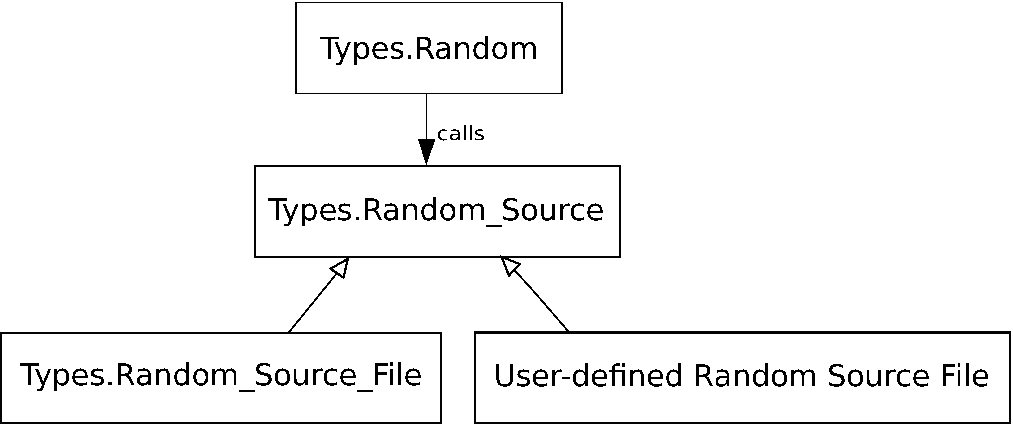
\includegraphics[scale=0.6]{./images/Random}
  \caption{The relationship among the data.}\label{WorkflowRandom}
\end{figure}
In the file \texttt{Random\_Source} the following abstract types and
procedures must be implemented:

\begin{lstlisting}{}
 package Fin renames Ada.Finalization;
 type Random_Source is abstract new Fin.Controlled with null record;
 type Random_Source_Access is access Random_Source;
 procedure Initialize(This: in out Random_Source) is abstract;
 procedure Read(This: in Random_Source; B: out Byte) is abstract;
\end{lstlisting}
When overwritting \texttt{Initialize()} in the file
\texttt{Random\_Source\_File}, the source path and source file are set
to "/dev/random" or some other user-defined random source. By calling
the procedure \texttt{Read()}, random bits are generated according to
the required type. After the reading procedure is finished, the source
file will be checked if it is closed, if it is open, then, a reading
error is raised.

%%%%%%%%%%%%%%%%%%%%%%%%%%%%%%%%%%%%%%%%%%%%%%%%%%%%%%%%%%%%%%%%%%
\section{"/dev/random"}\label{DevRandom}
In Linux, \texttt{Types.Random\_Source.File} assigns
\texttt{/dev/random} as the source file address by default. The device
node \texttt{/dev/random} can be seen as a special file that serves as
a random number generator or as a pseudorandom number
generator. Environmental noise will be gathered from device drivers
and other sources into an entropy pool, and then random numbers are
created \cite{dev-random}. When required, the \texttt{/dev/random} device
returns only bytes within the estimated number of bits of noise in the
entropy pool \cite{dev-random}.

If your operating system doesn't support \texttt{/dev/random} device, you can
install EGD (Entropy Gathering Daemon) by Brian Warners at the website
\textit{http://www.lothar.com/tech/cr\-ypto/}, it is a user-space
implementation of Linux-Kernel-Device \texttt{/dev/random}.

As mentioned in Section \ref{BasicRandom} the private part includes a
''Path'' variable. This variable indicates the path to a file, a named
pipe or a device storing cryptographically secure random
bits. Moreover, you can even link the ACL to a cryptographically
secure pseudorandom bit source on non-POSIX (Portable Operating System
Interface X) compliant operating systems, such as Windows XP.

%%%%%%%%%%%%%%%%%%%%%%%%%%%%%%%%%%%%%%%%%%%%%%%%%%%%%%%%%%%%%%%%%%

\subsection*{Example}
\begin{lstlisting}{}
   ...
   use Crypto.Types.Random_Source.File;
   Dev_U_Rand : Random_Source_File;
 begin
   Dev_U_Rand.Initialize("/dev/urandom");
   Crypto.Types.Random.Set(Dev_U_Rand);
   ...
\end{lstlisting}
